\section{Nanoribbons}
\label{sec:nanoribbon}

In this section, we apply our code to the case of honeycomb lattices with boundary conditions corresponding to nanoribbons. These structures are much longer on one direction than on the other, resembling a ribbon, hence their name.
The low energy electronic states on the edges of this ribbon might lead to interesting magnetic behavior in \ac{TMD} nanostructures (as indeed they do in graphene nanostructures \cite{yazyev_emergence_2010}) and it is this possibility was unexplored numerically before this work \cite{feldner_dynamical_2011, golor_quantum_2013}, as was mentioned on chapter \ref{cap:int}.
A nanoribbon is much longer on one direction than on the other, i.e. $l \gg w$. 
This condition corresponds to taking $N_x \gg N_y$ in our conventions (see Fig.(\ref{fig:nanoribbon}), where this condition is, of course, not obeyed solely for the sake of giving a good visual representation of the boundary conditions, and the numbering system).

\subsection{Graphene}
\label{sec:graphene}

We use three coordinates to label each site on the honeycomb lattice, by taking advantage of its bipartite nature.
Regarding the honeycomb lattice as two interpenetrating triangular sublattices $\mathcal{A}$ and $\mathcal{B}$, we take the axes $x$ and $y$ to be along the primitive vectors of each triangular sublattice.
Along the $x$-direction, the ribbon is supposed to be very long, which justifies the fact that we take \acp{PBC}.
In contrast, in the narrow $y$-direction we take \acp{OBC}.
To number the sites on the ribbon, we introduce an additional coordinate labeling the sublattice: $z = 0$, if the site is in sublattice $\mathcal{A}$, and $z = 1$ if the site is in sublattice $\mathcal{B}$.
We then adopt the numbering convention for the sites $i = 0,1, ..., 2 N_x N_y - 1$ of the lattice $\mathcal{L}$:

\begin{equation}\label{eq:numbering}
i (x, y, z) = N_x N_y z + N_x y + x,
\end{equation}
where $x = 0, ..., N_x - 1$, $y = 0, ..., N_y - 1$, and $z = 0, 1$ define each element $\bm r = (x, y, z) \in \mathcal{L}$.

\begin{figure}[H]\label{fig:bcRibbon}
	\centering
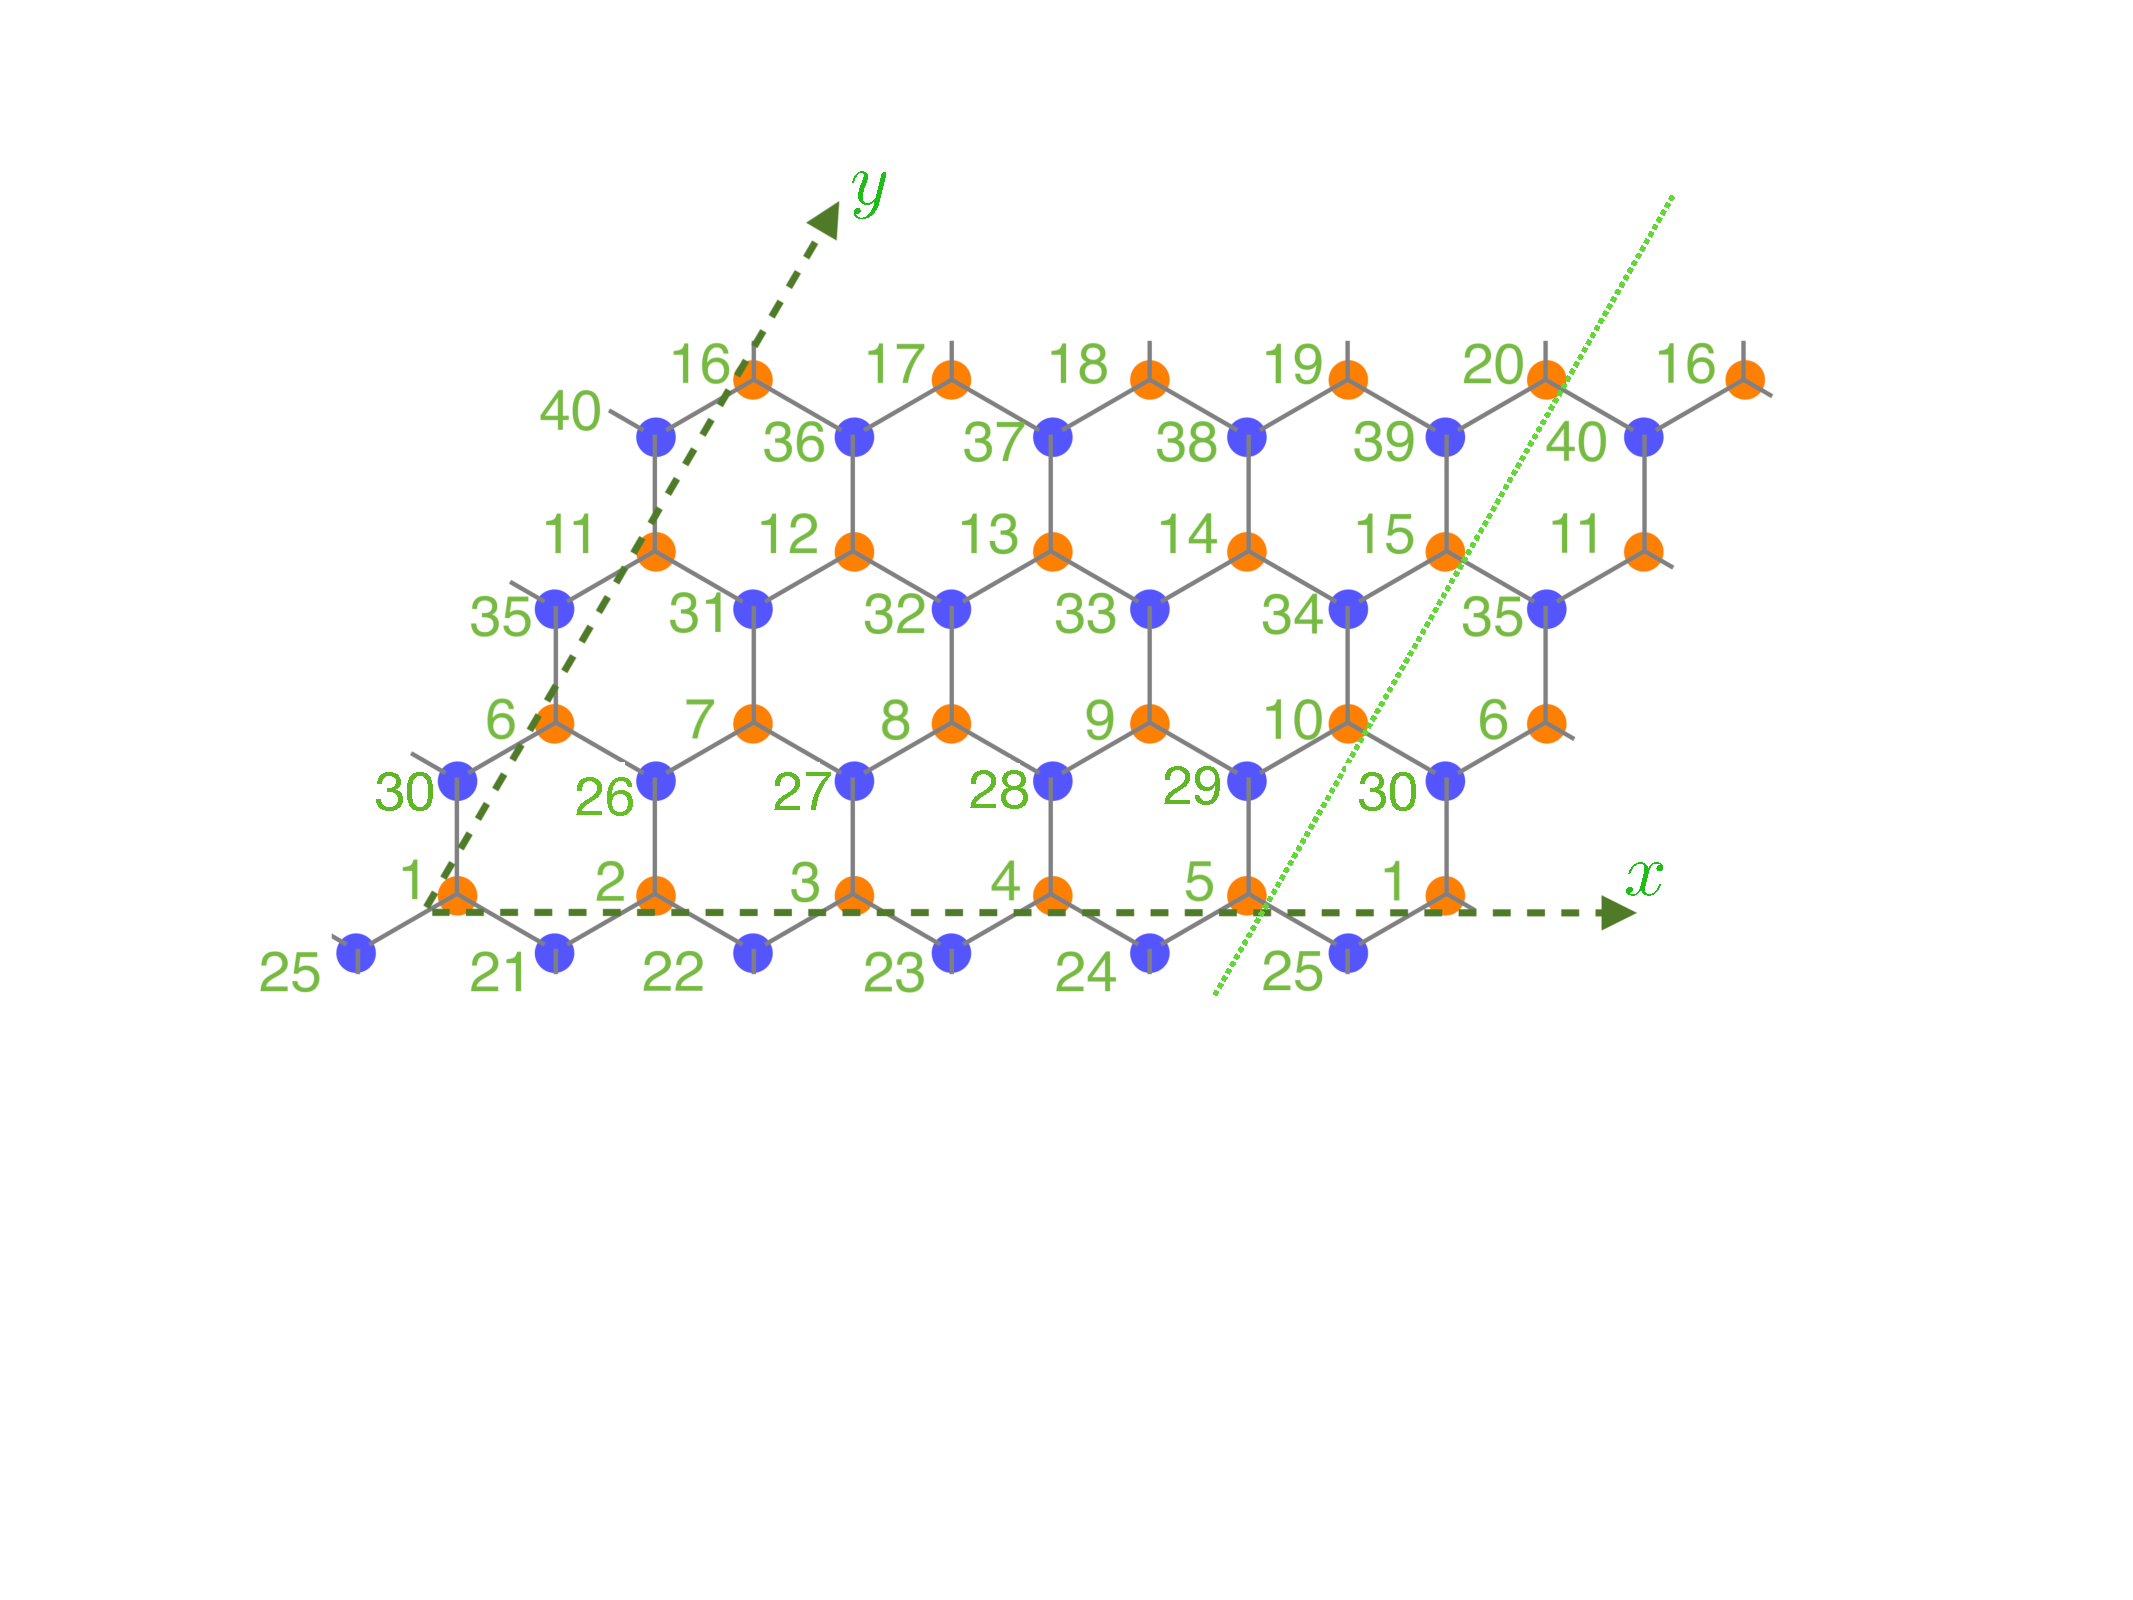
\includegraphics[trim={0 8cm 0 2.5cm},clip, width=0.8\linewidth]{Applications/nanoribbon.pdf}
	\caption[Boundary conditions on the nanoribbon.]{Boundary conditions on the nanoribbon for $N_x = 5, \, N_y = 4$. The orange circles correspond to sublattice $\mathcal{A}$, and the blue circles correspond to sublattice $\mathcal{B}$.
	The counting starts at 1 (i.e. the numbers correspond to $i+1$, since $i$ starts at 0).}
	\label{fig:nanoribbon}
\end{figure}

The geometry of the system appears through the hopping matrix $\bm K$ in our code.
This numbering system makes it straightforward to find the neighbors of each site.
Let us begin by considering a site that is not on a zigzag edge.
There are two possible cases. For example, for 

\begin{equation*}
z_i = 0, y_i \neq N_y - 1, x_i \neq 0 ,
\end{equation*}
we have that the nearest neighbors of $i$ are $ j (i) = \{ j ( \bm r) \}$, with $\bm r$ in
\begin{equation*}
\bigg\{ \bm r_j \in \mathcal{L} \bigg| z_j = 1 \,\land\, \bigg[ \bigg( y_j = y_i  \,\land\, ( x_j = x_i \,\lor\, x_j = x_i - 1) \bigg) \,\lor\, \bigg( y_j = y_i + 1  \,\land\, x_j = x_i - 1  \bigg)  \bigg] \bigg\}
\end{equation*}

As opposed to the sites of a honeycomb lattice with \acp{PBC}, which have 3 neighbors, the sites of the zigzag edges have only 2 neighbors.
We summarize all possible cases in the following table.

\begin{table}[H]
\centering
	\caption{Nearest neighbors on the graphene nanoribbon.
	The neighbors in gray are only for sites that are not on the edges.
	$\%$ refers to the remainder of integer division.}
	\begin{tabular}{|c|c|c|c|} \hline
	\multicolumn{4}{|c|}{\textbf{\acp{OBC} \color{silver}{(\acp{PBC})} }}							\\ \hline
		Case 				& $z_j$	& $y_j$	& $x_j$ 	\\ \hline
		\multicolumn{1}{|c|}{\multirow{3}{*}{$z_i = 0$}}	 &	\multicolumn{1}{c|}{\multirow{3}{*}{1}} & \multicolumn{1}{c|}{\multirow{2}{*}{$y_i$}} & $x_i$   \\ \cline{4-4}
	   	\multicolumn{1}{|c|}{}	& \multicolumn{1}{c|}{\multirow{3}{*}{}} & \multicolumn{1}{c|}{\multirow{2}{*}{}}& \multicolumn{1}{c|}{\multirow{2}{*}{$N_x - 1 - (N_x - x_i) \% N_x$}} \\ \cline{3-3}
	   	\multicolumn{1}{|c|}{}	& \multicolumn{1}{c|}{} & \color{silver}{$y_i +1$} & \multicolumn{1}{c|}{\multirow{2}{*}{}} \\ \hline
%		\multicolumn{1}{|c|}{\multirow{3}{*}{$z_i = 0, y_i \neq N_y - 1, x_i = 0$}}	 &	\multicolumn{1}{c|}{\multirow{3}{*}{1}} & \multicolumn{1}{c|}{\multirow{2}{*}{$y_i$}} & 0   \\ \cline{4-4}
%	   	\multicolumn{1}{|c|}{}	& \multicolumn{1}{c|}{\multirow{3}{*}{}} & \multicolumn{1}{c|}{\multirow{2}{*}{}}& \multicolumn{1}{c|}{\multirow{2}{*}{$N_x - 1$}} \\ \cline{3-3}
%	   	\multicolumn{1}{|c|}{}	& \multicolumn{1}{c|}{} & $y_i +1$ & \multicolumn{1}{c|}{\multirow{2}{*}{}} \\ \hline
		\multicolumn{1}{|c|}{\multirow{3}{*}{$z_i = 1$}}	 &	\multicolumn{1}{c|}{\multirow{3}{*}{0}} & \multicolumn{1}{c|}{\multirow{2}{*}{$y_i$}} & $x_i$   \\ \cline{4-4}
	   	\multicolumn{1}{|c|}{}	& \multicolumn{1}{c|}{\multirow{3}{*}{}} & \multicolumn{1}{c|}{\multirow{2}{*}{}}& \multicolumn{1}{c|}{\multirow{2}{*}{$(x_i + 1) \% N_x$}} \\ \cline{3-3}
	   	\multicolumn{1}{|c|}{}	& \multicolumn{1}{c|}{} & \color{silver}{$y_i -1$} & \multicolumn{1}{c|}{\multirow{2}{*}{}} \\ \hline
%		\multicolumn{1}{|c|}{\multirow{3}{*}{$z_i = 1$, $y_i \neq 0$, $x_i = N_x - 1$}}	 &	\multicolumn{1}{c|}{\multirow{3}{*}{0}} & \multicolumn{1}{c|}{\multirow{2}{*}{$y_i$}} & $N_x - 1$   \\ \cline{4-4}
%	   	\multicolumn{1}{|c|}{}	& \multicolumn{1}{c|}{\multirow{3}{*}{}} & \multicolumn{1}{c|}{\multirow{2}{*}{}}& \multicolumn{1}{c|}{\multirow{2}{*}{0}} \\ \cline{3-3}
%	   	\multicolumn{1}{|c|}{}	& \multicolumn{1}{c|}{} & $y_i -1$ & \multicolumn{1}{c|}{\multirow{2}{*}{}} \\ \hline
	\end{tabular}
%	\hspace{-0.1cm}
%	\begin{tabular}{|c|c|c|c|} \hline
%	\multicolumn{4}{|c|}{\textbf{\acp{OBC}}}							\\ \hline
%		Case 				& $z_j$	& $y_j$	& $x_j$ 	\\ \hline
%	\multicolumn{1}{|c|}{\multirow{2}{*}{$z_i = 0, y_i = N_y - 1$}}	 &	\multicolumn{1}{c|}{\multirow{2}{*}{1}} & \multicolumn{1}{c|}{\multirow{2}{*}{$y_i$}} & $x_i$   \\ \cline{4-4}
%	   	\multicolumn{1}{|c|}{}	& \multicolumn{1}{c|}{\multirow{2}{*}{}}  & \multicolumn{1}{c|}{}& $N_x - 1 - (N_x - x_i) \% N_x$ \\ \hline
%	   	\multicolumn{1}{|c|}{\multirow{2}{*}{$z_i = 0, y_i = N_y - 1, x_i = 0$}}	 &	\multicolumn{1}{c|}{\multirow{2}{*}{1}} & \multicolumn{1}{c|}{\multirow{2}{*}{$y_i$}} & 0   \\ \cline{4-4}
%	   	\multicolumn{1}{|c|}{}	& \multicolumn{1}{c|}{\multirow{2}{*}{}}  & \multicolumn{1}{c|}{}& $N_x - 1$ \\ \hline
%	   	\multicolumn{1}{|c|}{\multirow{2}{*}{$z_i = 1, y_i = 0$}}	 &	\multicolumn{1}{c|}{\multirow{2}{*}{0}} & \multicolumn{1}{c|}{\multirow{2}{*}{$y_i$}} & $x_i$   \\ \cline{4-4}
%	   	\multicolumn{1}{|c|}{}	& \multicolumn{1}{c|}{\multirow{2}{*}{}}  & \multicolumn{1}{c|}{}& $(x_i + 1) \% N_x$  \\ \hline
%	   	\multicolumn{1}{|c|}{\multirow{2}{*}{$z_i = 1, y_i = 0, x_i = N_x - 1$}}	 &	\multicolumn{1}{c|}{\multirow{2}{*}{0}} & \multicolumn{1}{c|}{\multirow{2}{*}{$y_i$}} & 0   \\ \cline{4-4}
%	   	\multicolumn{1}{|c|}{}	& \multicolumn{1}{c|}{\multirow{2}{*}{}}  & \multicolumn{1}{c|}{}& $N_x - 1$ \\ \hline
%	\end{tabular}
	\label{tab:dummytable}
\end{table}

\subsection{\acp{TMD}}
\label{subsec:apTMD}

We start by approaching the \acs{TMDNR} problem at the mean field level.
Such a procedure allows one to understand the system in a simplified manner that is very useful to obtain a crude picture of its behavior.
In particular, if there is a transition between a configuration with magnetic order, and a disordered one, there is a critical interaction parameter $U = U_c$ at which the transition occurs, and it can be estimated in mean field, and compared with the more precise \acs{QMC} result.
In general, our mean field formulation would involve diagonalizing an $N \times N$ matrix at each step, where $N = N_{\text{orb}} N_x N_y$ is the size of the system times the number of orbitals.
However, since we consider \acs{PBC}s along the $x$-direction, we can partially diagonalize  the Hamiltonian analytically, reducing the size of the matrix to be diagonalized to $3 N_y \times 3 N_y$, where $N_y$ is the width of the ribbon, i.e. the number of $\text{M}\text{X}_2$ formula units.
Consider the spinless 3-band tight binding model, with the normalized lattice constant: $a = 1$.

\begin{equation}
\begin{split}
\mathcal{H}_0 &= \sum_{\substack{m, n \\ \alpha, \beta}} \bigg( c_{m,n, \alpha}^\dagger t_{\alpha\beta}^0 c_{m, n, \beta} + \delta_{0, N_x}  c_{m,n, \alpha}^\dagger t_{\alpha\beta}^1 c_{m+1, n, \beta} + \delta_{-\sqrt{3}/2, (N_y -1)\sqrt{3}/2}  c_{m,n, \alpha}^\dagger t_{\alpha\beta}^4 c_{m-1, n, \beta} \\
& + \delta_{0, N_m} \delta_{-1, (N_y -1)\sqrt{3}/2} c_{m+1/2,n-\sqrt{3}/2, \alpha}^\dagger t_{\alpha\beta}^2 c_{m, n, \beta} + \delta_{-1, (N_y -1)\sqrt{3}/2} c_{m-1/2,n-\sqrt{3}/2, \alpha}^\dagger t_{\alpha\beta}^3 c_{m, n, \beta} \\
& + \delta_{N_y\sqrt{3}/2, 0} c_{m+1/2,n+\sqrt{3}/2, \alpha}^\dagger t_{\alpha\beta}^6 c_{m, n, \beta} + \delta_{-1, N_x -1} \delta_{N_y\sqrt{3}/2, 0} c_{m-1/2,n+\sqrt{3}/2, \alpha}^\dagger t_{\alpha\beta}^5 c_{m, n, \beta} \bigg)
\end{split}
\end{equation}

Fourier transforming in $x$: $c_{m, n, \alpha} = \frac{1}{\sqrt{N_x}}\sum_{k} e^{-i k m } c_{k, n, \alpha} $, with $k = \frac{2\pi}{N_x} \{ -\frac{N_x}{2} + 1, -\frac{N_x}{2}, ..., \frac{N_x}{2} \}$:

\begin{equation}
\begin{split}
\mathcal{H}_0 &= \sum_{ \substack{k, y \\ \alpha, \beta} } \bigg( c_{k, y, \alpha}^\dagger (t_{\alpha \beta}^0  + e^{ik} t_{\alpha \beta}^1 + e^{-ik} t_{\alpha \beta}^4 )  c_{k, y, \beta} + \delta_{-1, N_y -1} c_{k, y - 1, \alpha}^\dagger ( e^{ik/2} t_{\alpha \beta}^2 + e^{-ik/2} t_{\alpha \beta}^3 ) c_{k, y, \beta} \\
& + \delta_{N_y, 0} c_{k, y, \alpha}^\dagger ( e^{ik/2} t_{\alpha \beta}^6 + e^{-ik/2} t_{\alpha \beta}^5 ) c_{k, y+1, \beta} \bigg) , \,\, \text{with} \, y \, \text{defined as in Fig.(4.1)}
\end{split}
\end{equation}
leading to a tridiagonal block $3 N_y \times 3 N_y$ hopping matrix $\bm H (k)$ with three different types of matrix elements: $\bm h_1 = \bm H_{y,y}$, $\bm h_2 = \bm H_{y,y-1}$, $\bm h_2^\dagger = \bm H_{y, y+1}$.

\begin{equation}
[ H_{(\alpha y) (\beta y')} (k) ] = 
\begin{pmatrix}
\bm h_1 & \bm h_2^\dagger & & & \\
\bm h_2 & \bm h_1 & \bm h_2^\dagger & & \\
& \bm h_2 & \bm h_1 & \ddots & \\
& & \ddots & \ddots & \bm h_2^\dagger \\
& & & \bm h_2 & \bm h_1
\end{pmatrix}, \, 
\bm h_1 = 
\begin{pmatrix}
\varepsilon_1 + 2 t_0 \cos k & 2 i t_1 \sin k & 2 t_2 \cos k \\
-2 i t_1 \sin k & \varepsilon_2 + 2 t_{11} \cos k & 2 i t_{12} \sin k \\
2 t_2 \cos k& -2 i t_{12} \sin k & \varepsilon_2 + 2 t_{22} \cos k \\
\end{pmatrix}
\end{equation}

\begin{equation*}
\bm h_2 =
\begin{pmatrix}
2 t_0 \cos ( k / 2 ) & i \sin ( k / 2 ) \bigg( t_1 - \sqrt{3} t_2 \bigg) & - \cos (k /2 ) \bigg( \sqrt{3} t_1 + t_2 \bigg) \\
-i \sin ( k / 2 ) \bigg(t_1 + \sqrt{3} t_2 \bigg) & \frac{1}{2} \cos (k / 2) \bigg( t_{11} + 3 t_{22} \bigg) & -i \sin (k / 2) \bigg( \frac{\sqrt{3}}{2} (t_{11} -  t_{22} ) + 2 t_{12} \bigg) \\
\cos ( k / 2) \bigg( \sqrt{3} t_1 - t_2 \bigg) & -i \sin (k / 2) \bigg( \frac{\sqrt{3}}{2} ( t_{11} - t_{22} ) - 2 t_{12} \bigg) & \frac{1}{2} \cos (k / 2) \bigg( 3 t_{11	} + t_{22} \bigg)
\end{pmatrix}
\end{equation*}

\begin{figure}[H]
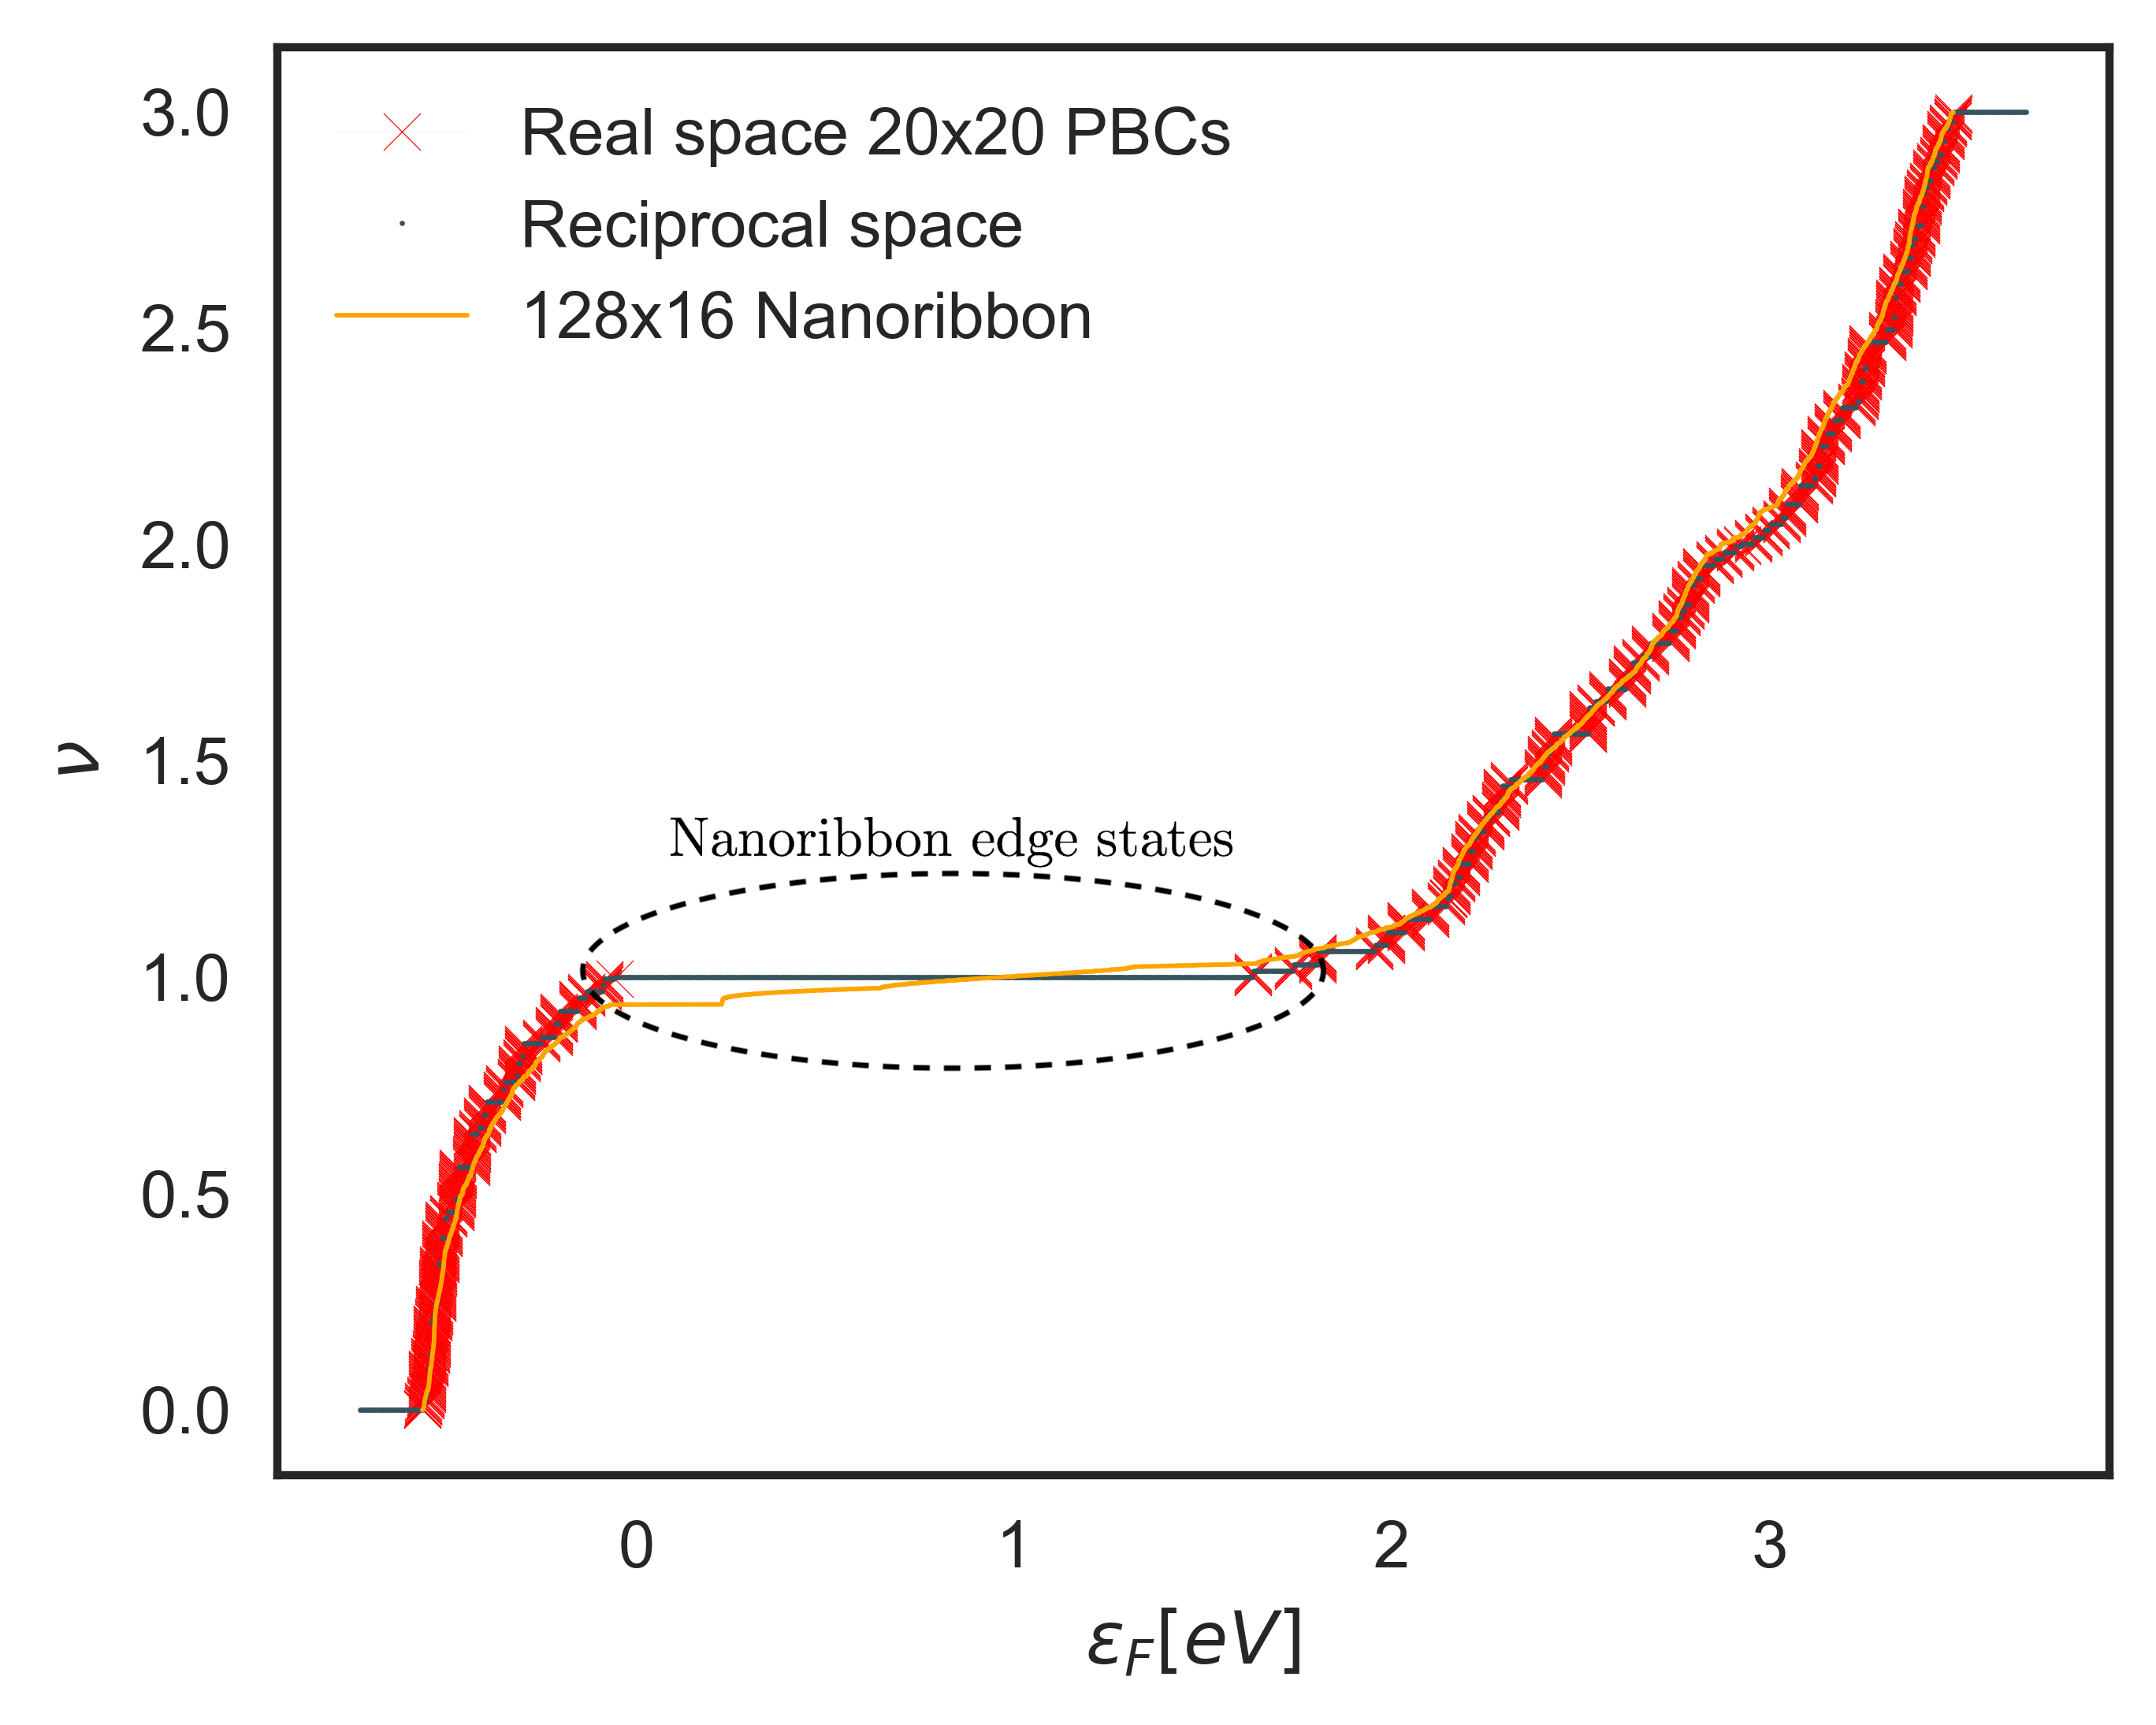
\includegraphics[scale=0.5]{Applications/fillingVsE.png}
\hspace{2cm}
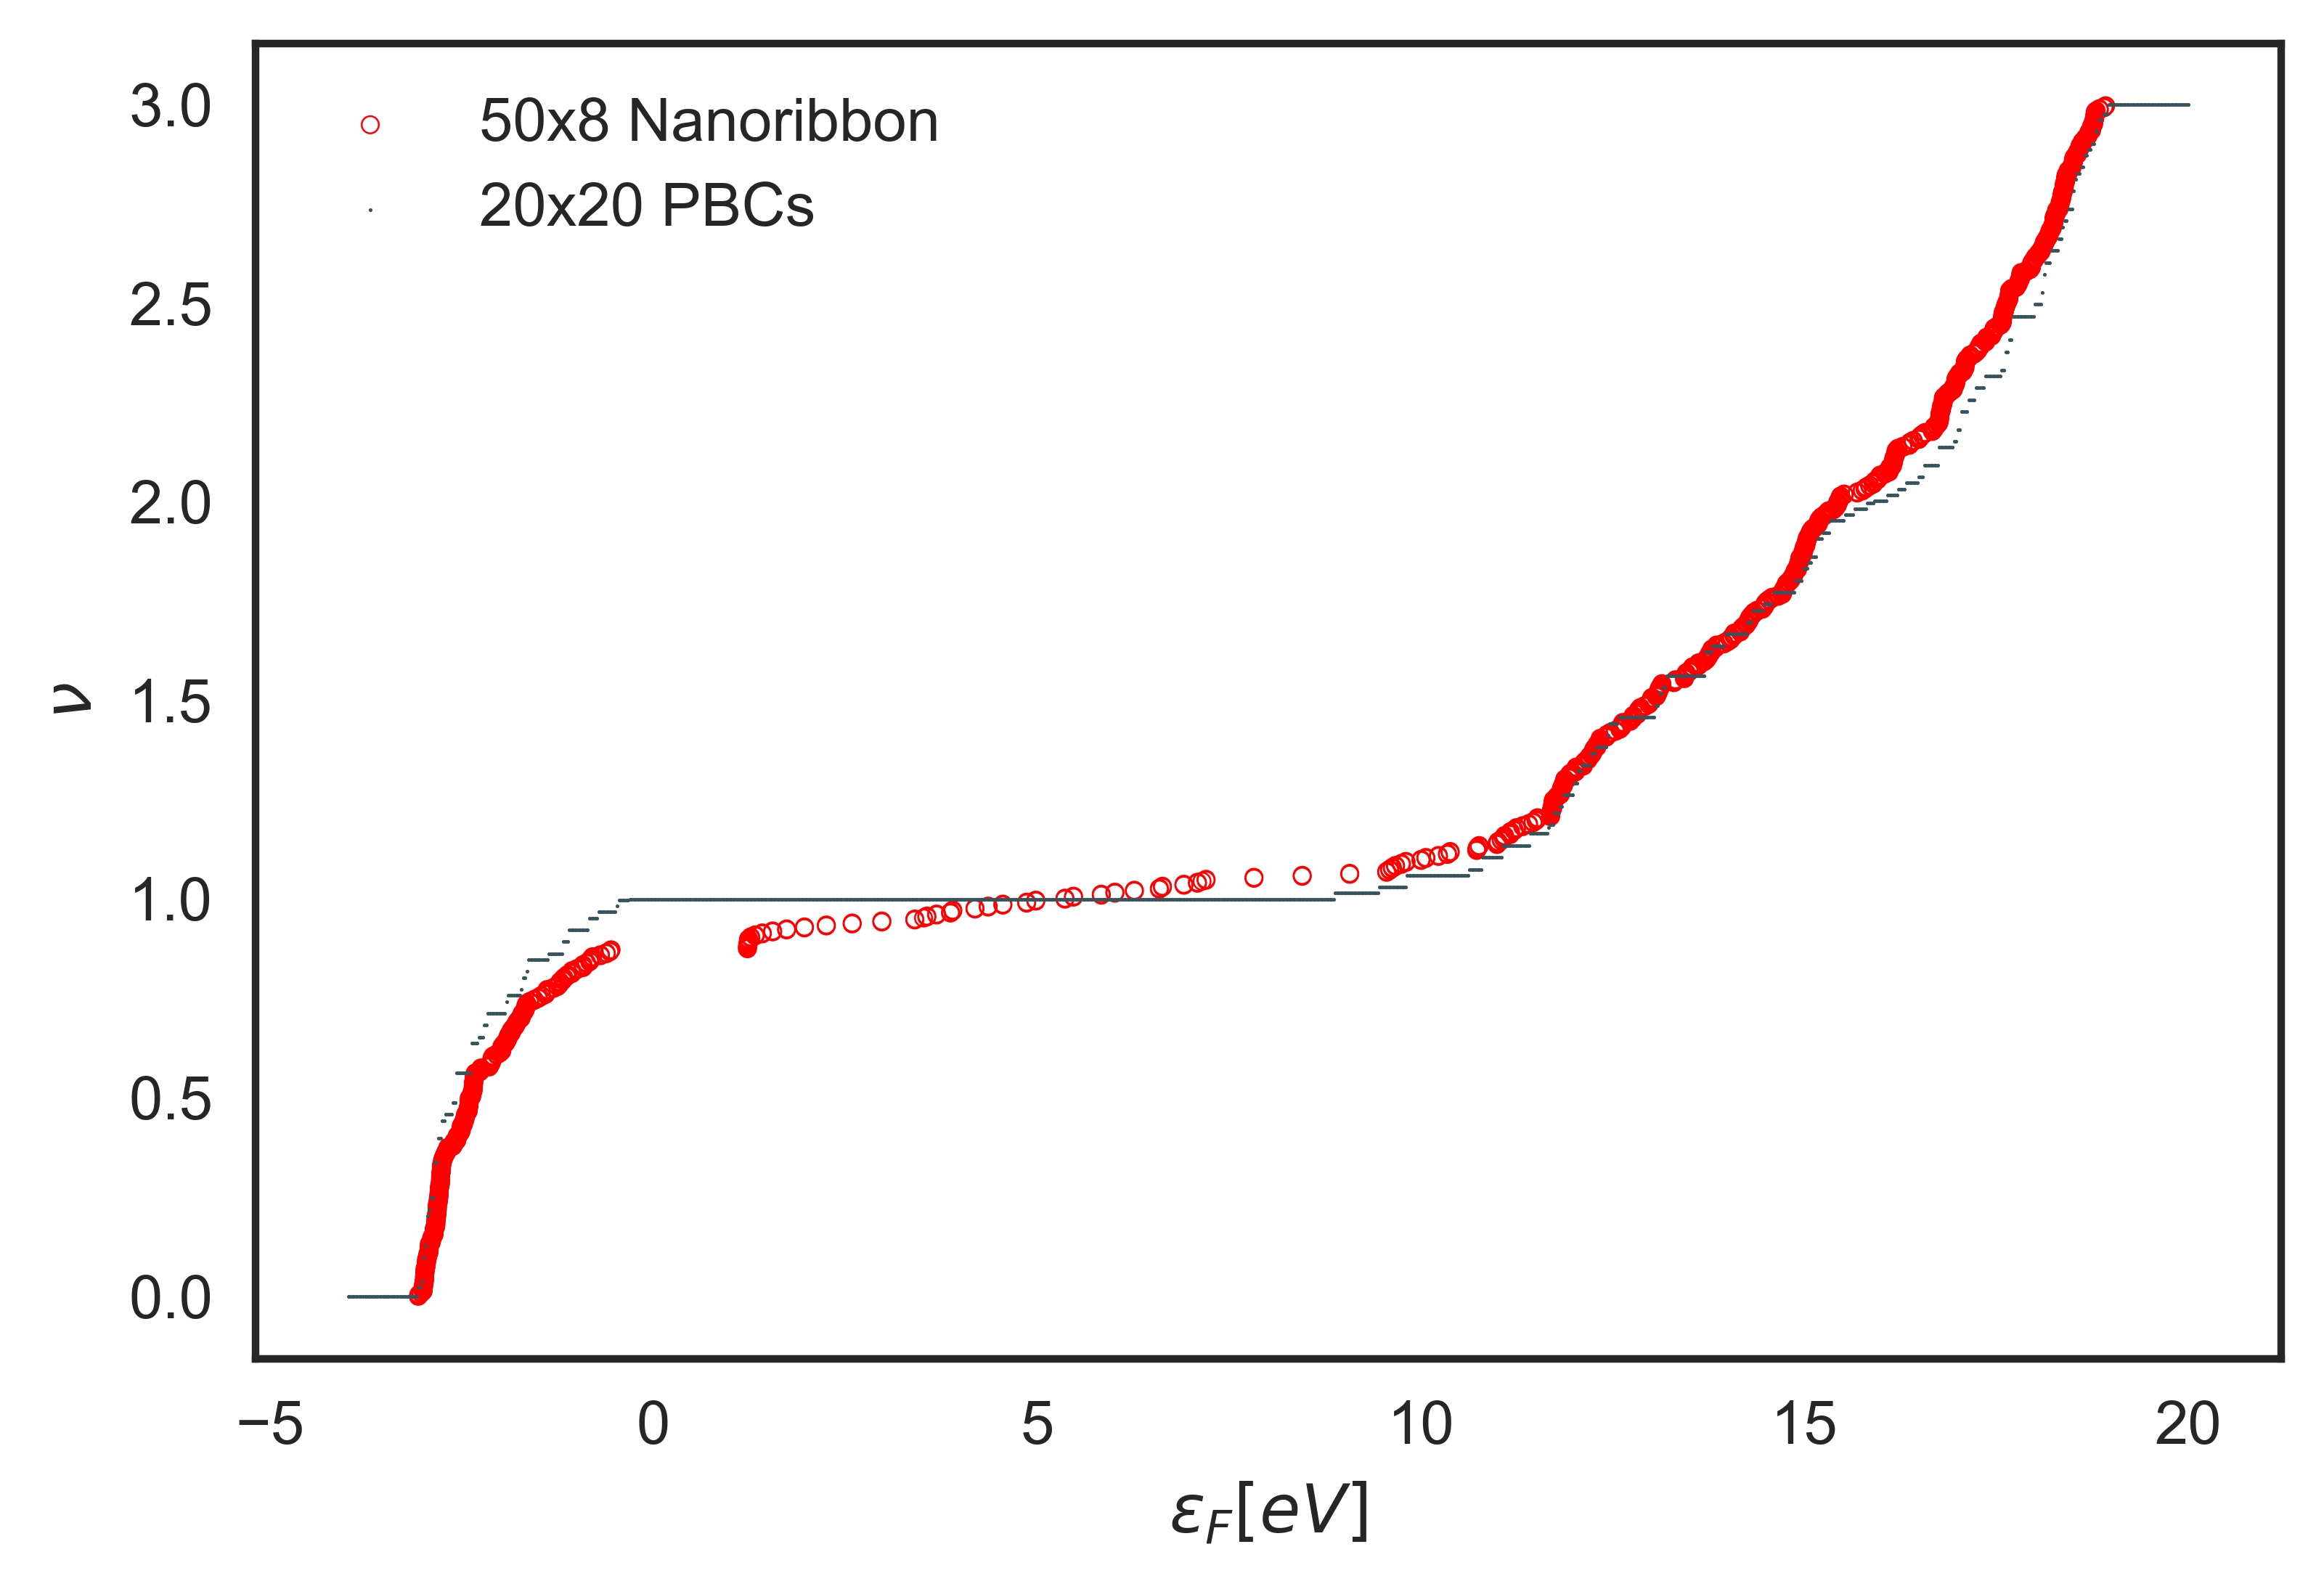
\includegraphics[scale=0.5]{Applications/fillingVsEnanoribbon.png}
	\caption[Filling factor as a function of the Fermi energy for \acs{TMD} monolayers and nanoribbons.]{Left: Filling factor as a function of the Fermi energy for a system with \acp{PBC}, as computed by diagonalizing the input matrix of our code, and by the hopping matrix in $\bm k$-space.
	Right: Comparison between the filling factors of a nanoribbon and a periodic system as a function of the Fermi energy, as computed by diagonalizing our input matrix. 
	For the nanoribbon, edge states appear on the gap of the periodic system.}
	\label{fig:fillingVsE}
\end{figure}

\begin{figure}[H]
\includegraphics[scale=0.26]{Applications/bandstruct}
\hspace{1.5cm}
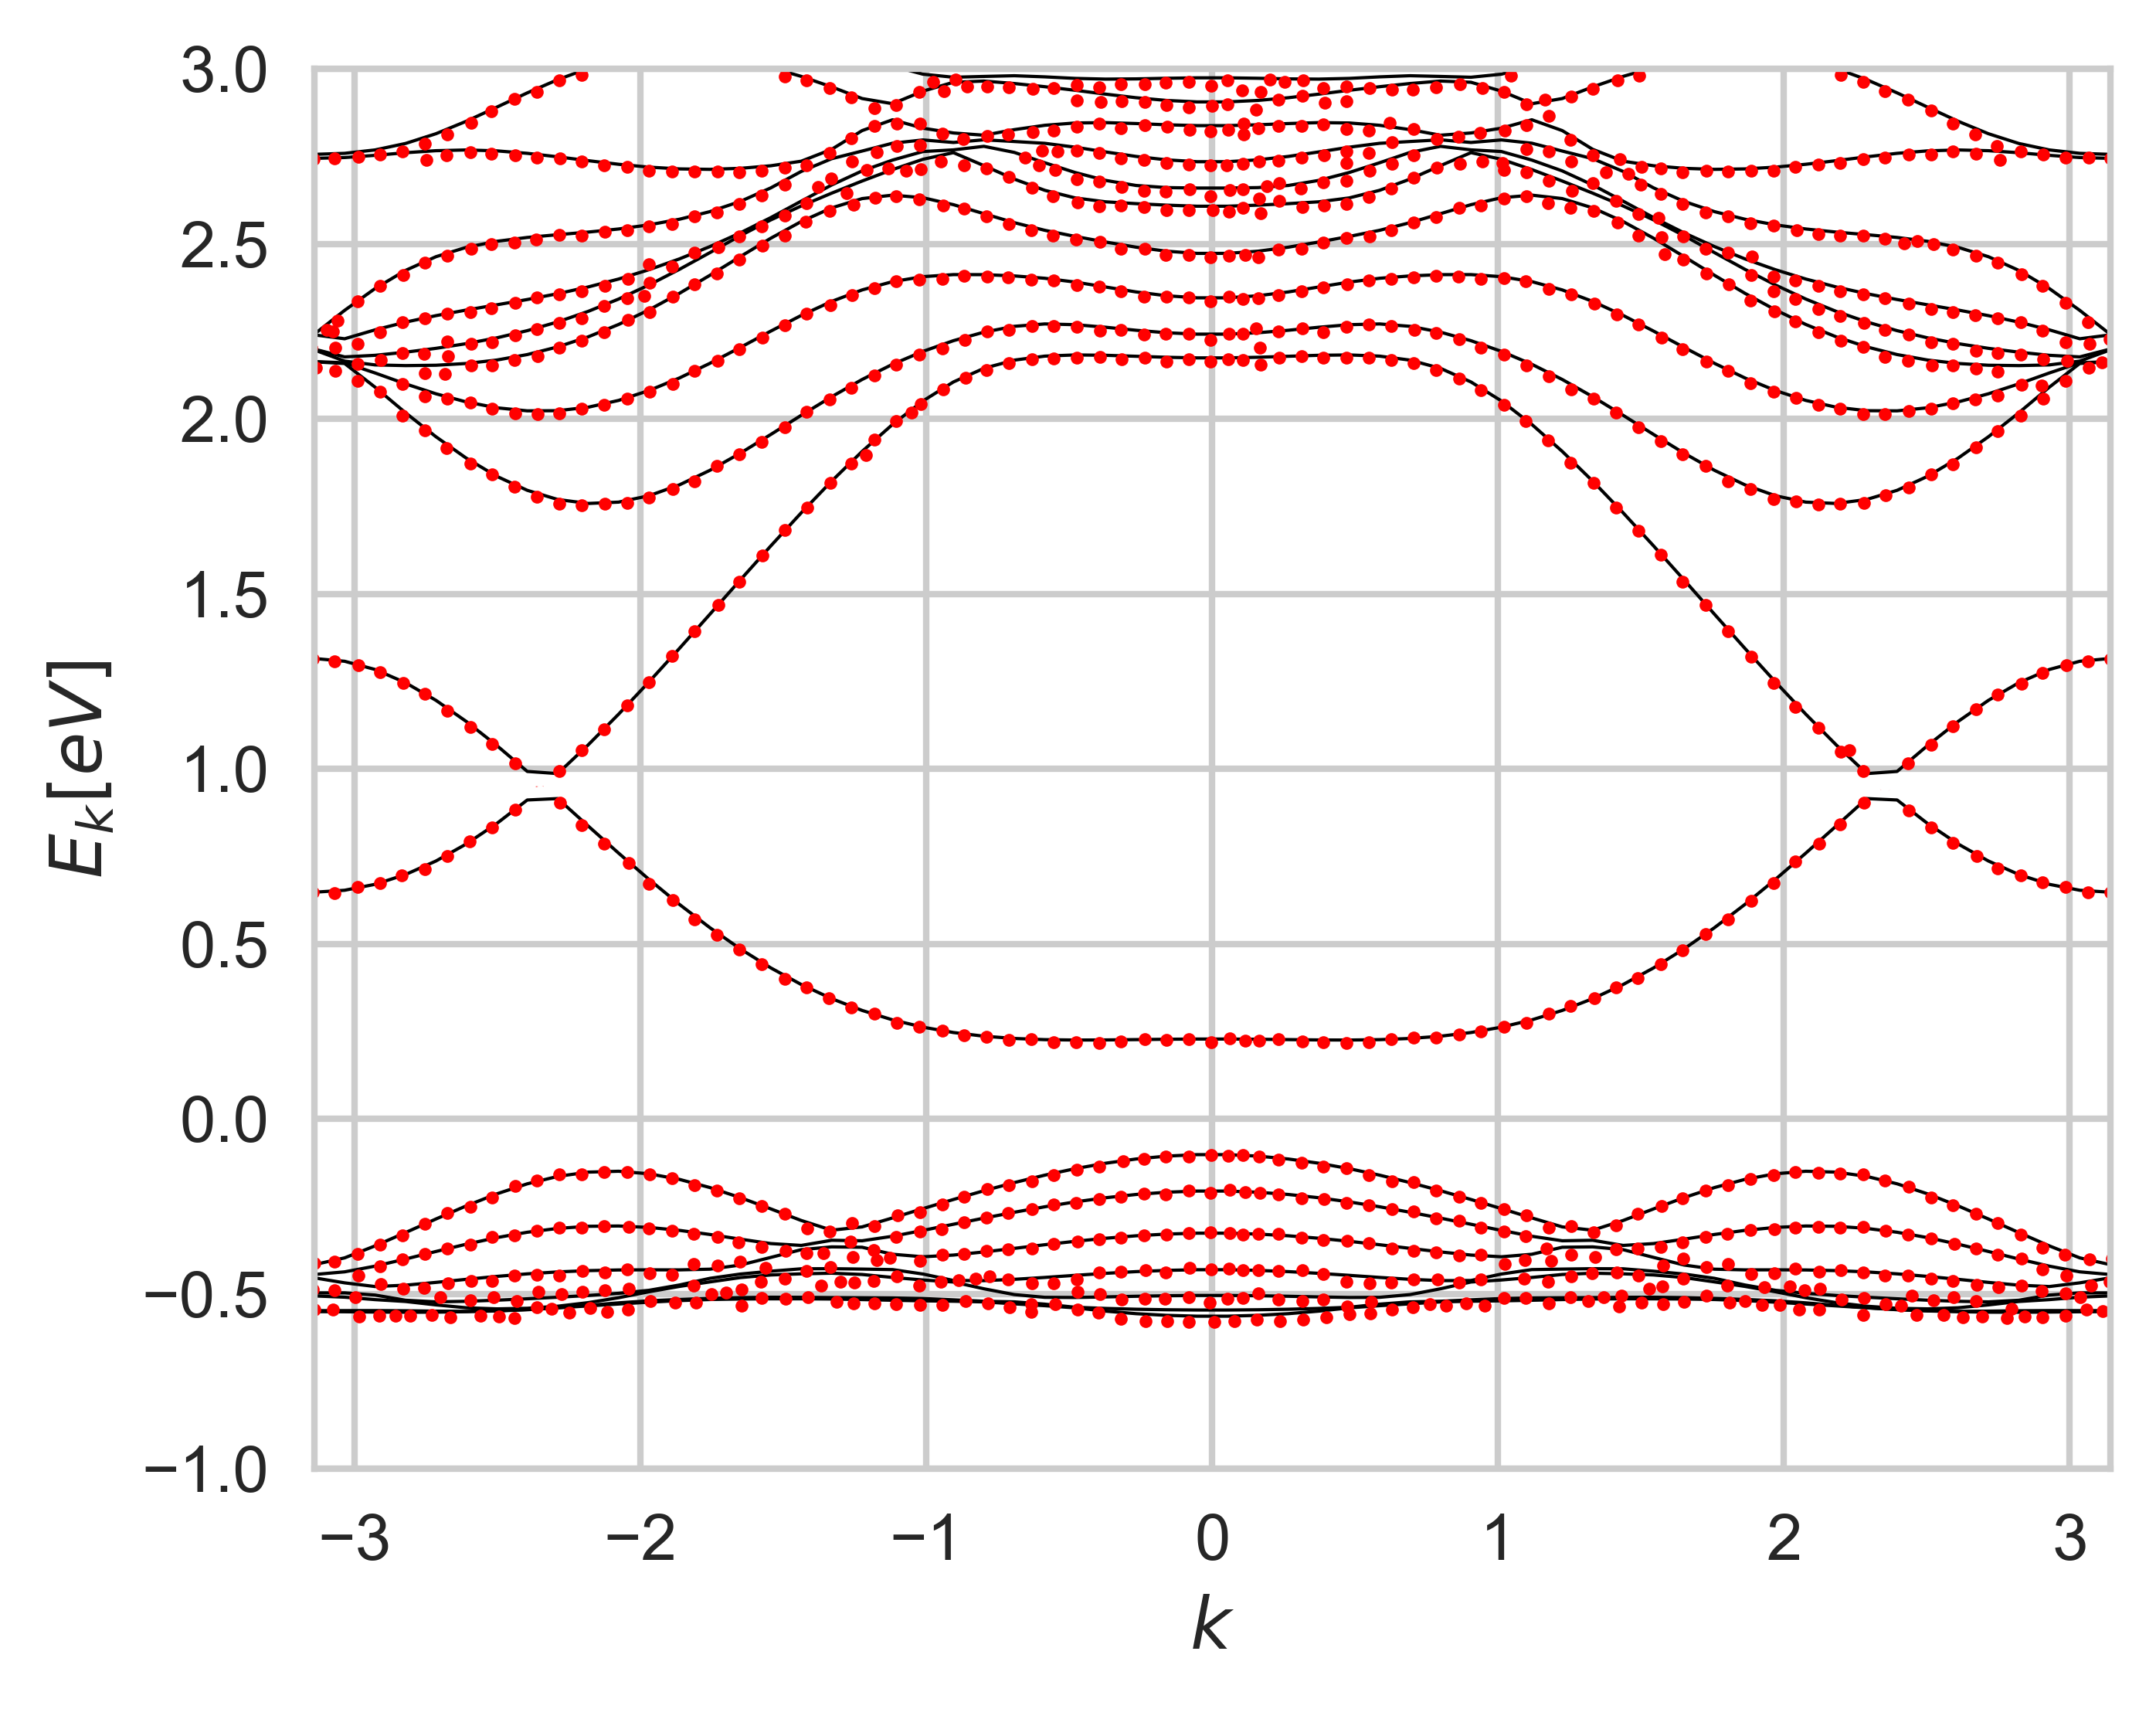
\includegraphics[scale=0.6]{Applications/BandStructureNanoribbonTMD.png}
	\caption[$\text{Mo}\text{S}_2$ \acs{TMDNR} band structure for $N_y = 8$, obtained by the 3-band model.]{Left: $\text{Mo}\text{S}_2$ zigzag edged nanoribbon energy bands (red dots), for $N_y = 8$, using the GCA parameters. The first principles bands show the contribution from orbitals that are not considered in the 3-band model (blue:  $d_{z^2}$, $d_{xy}$, $d_{x^2-y^2}$, green: others). The model reproduces the bands that correspond to the orbitals taken into account reasonably (1 and 2 correspond to the edge states from the $d_{z^2}$, $d_{xy}$, $d_{x^2-y^2}$ orbitals of the $\text{Mo}$ atoms, while 3 and 4 correspond to the $d_{yz}$ orbital at the $\text{Mo}$-terminated edge, and $p_{y, z}$ orbitals from the $\text{S}$-terminated edge, and are not taken into account in the 3-band model). Right: Band structure obtained by us (black) from the 3-band model  reproducing the result on the left (red dots,  extracted by \texttt{WebPlotDigitizer}.) \cite{liu_three-band_2013}.}
	\label{fig:bandStruct}
\end{figure}

By applying our mean field approach to solve the 3-band model with Hubbard-type interactions, we obtain solutions that are independent of $x$, which motivates us to reduce the number of MF parameters by choosing a translationally invariant ansatz.
This is equivalent to taking $\left\langle n_{x, y,\alpha, \sigma}\right\rangle = \left\langle n_{y,\alpha, \sigma}\right\rangle  \forall x$ ($6 N_y$ parameters).
By reducing the number of parameters, convergence is facilitated, which allows us to evaluate whether the solution of Fig.(\ref{fig:nanoGraphVsTMD}) is robust, i.e. whether it corresponds to a metastable or not.
The mean field form of the interaction term with the reduced number of parameters changes, implying that the self-consistent relation of Eq.(\ref{eq:selfConsistent}) from which the local densities are computed changes as well.

\begin{equation}
\mathcal{H}_{\text{MF}} = \mathcal{H}_0 + \mathcal{H}_1 , \,\text{where} \,\, \mathcal{H}_1 = U \sum_{m, n, \alpha} \bigg( \sum_\sigma n_{\substack{m, \sigma \\ n, \alpha}} \big\langle n_{\substack{m, -\sigma \\ n, \alpha}} \big\rangle  - \big\langle n_{\substack{m, \uparrow \\ n, \alpha}} \big\rangle \big\langle n_{\substack{m, \downarrow \\ n, \alpha}} \big\rangle \bigg)
\end{equation}

\begin{equation}
\begin{split}
\mathcal{H}_1 &= \frac{U}{N_x^{\,2}} \sum_{\substack{n \alpha \\ k_1 k_2 \\ k_3 k_4}} \underbrace{\sum_m e^{i [ (k_1 + k_3) - (k_2 + k_4) ] m}}_{N_x \delta_{k_4, k_1 + k_3 - k_2}} \bigg( \sum_\sigma c_{\substack{k_1, \sigma \\ n, \alpha}}^\dagger c_{\substack{k_2, \sigma \\ n, \alpha}} \underbrace{\big\langle c_{\substack{k_3, -\sigma\\ n, \alpha}}^\dagger c_{\substack{k_4, -\sigma \\ n, \alpha}} \big\rangle}_{\delta_{k_3, k_4} \big\langle n_{\substack{k_3,-\sigma \\ n, \alpha}} \big\rangle} - \underbrace{\big\langle c_{\substack{k_1, \uparrow \\ n, \alpha}}^\dagger c_{\substack{k_2  \uparrow \\n, \alpha}} \big\rangle}_{\delta_{k_1, k_2} \big\langle n_{\substack{k_2,\uparrow \\ n, \alpha}} \big\rangle} \underbrace{\big\langle c_{\substack{k_3, \downarrow \\ n, \alpha}}^\dagger c_{\substack{k_4, \downarrow \\ n, \alpha}} \big\rangle}_{\delta_{k_3, k_4} \big\langle n_{\substack{k_3,\downarrow \\ n, \alpha}} \big\rangle}  \bigg) \\
&= \frac{U}{N_x} \sum_{\substack{n \alpha \\ k_2 k_3}} \bigg( \sum_\sigma n_{\substack{k_2, \sigma \\ n, \alpha}} \big\langle n_{\substack{k_3, -\sigma \\ n, \alpha}} \big\rangle - \big\langle n_{\substack{k_2, \uparrow \\ n, \alpha}} \big\rangle \big\langle n_{\substack{k_3, \downarrow \\ n, \alpha}} \big\rangle \bigg) \equiv
U \sum_{\mu,k} \bigg( \sum_\sigma n_{\mu, k,\sigma} \big\langle n_{\mu, -\sigma} \big\rangle - \big\langle n_{\mu, \uparrow} \big\rangle \big\langle n_{\mu, \downarrow} \big\rangle \bigg)
\end{split}
\end{equation}
where we collapsed the indexes $(n, \alpha)$ into a single index $\mu$.
The self consistent relation allowing us to compute the new MF parameters at each step emerges by diagonalizing $\mathcal{H}_1$ in the $\mu$-subspace:

\begin{equation}
\big\langle n_{\mu, \sigma} \big\rangle = \frac{1}{N_x}\sum_{q, \gamma} | Q_{q \sigma \mu, \gamma} |^2 \rho ( \varepsilon_{q \gamma \sigma} ) , \, \text{where} \, d_{q, \sigma, \gamma} = \sum_\gamma Q_{q \sigma \mu, \gamma}^\star c_{q ,\sigma, \mu} ,  \, \text{and} \,\, \mathcal{H}_{\text{MF}} = \sum_{k, \gamma, \sigma} \varepsilon_{k, \gamma, \sigma} d_{q, \sigma, \gamma}^\dagger d_{q, \sigma, \gamma} + \text{const.}
\end{equation}

\begin{figure}[H]
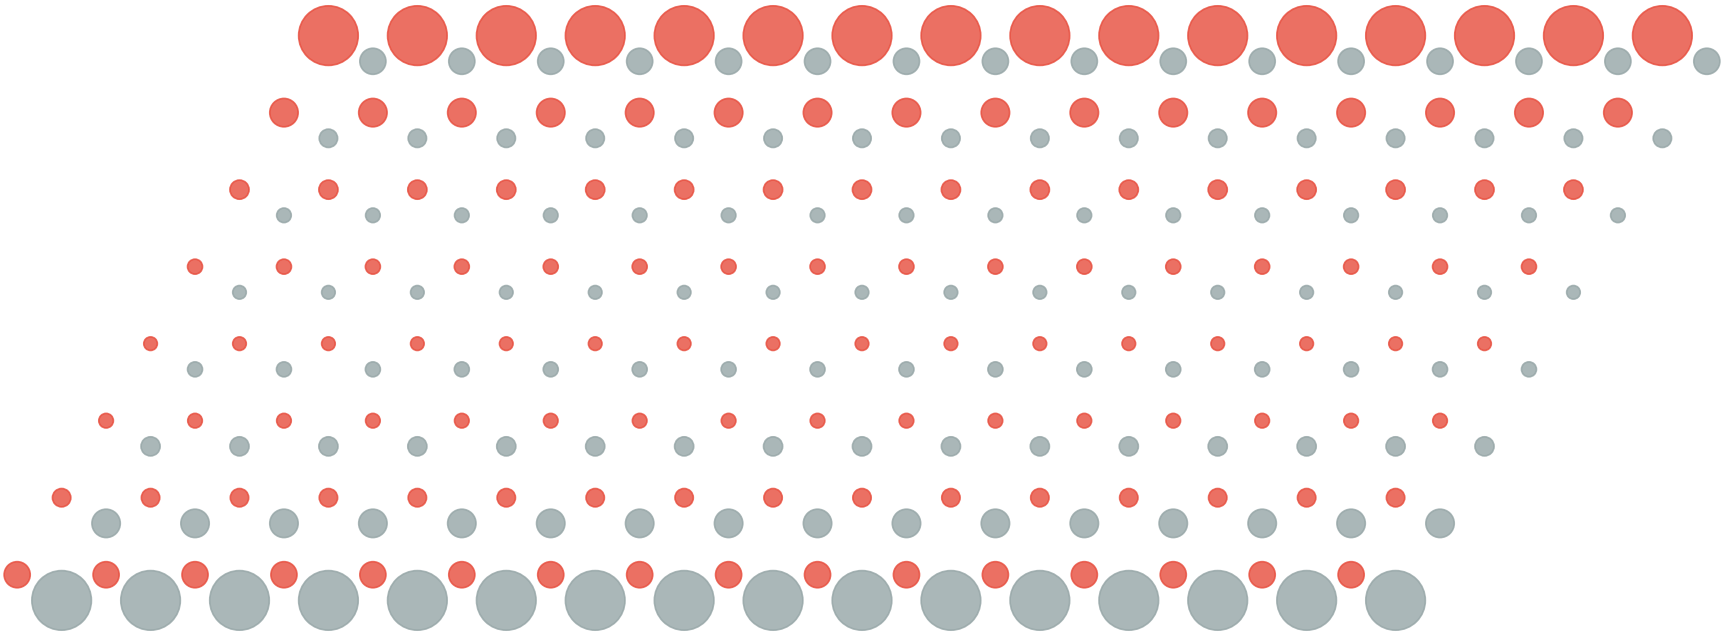
\includegraphics[scale=0.5]{Applications/MFnanoribbon.png}
\hspace{-0.18cm}
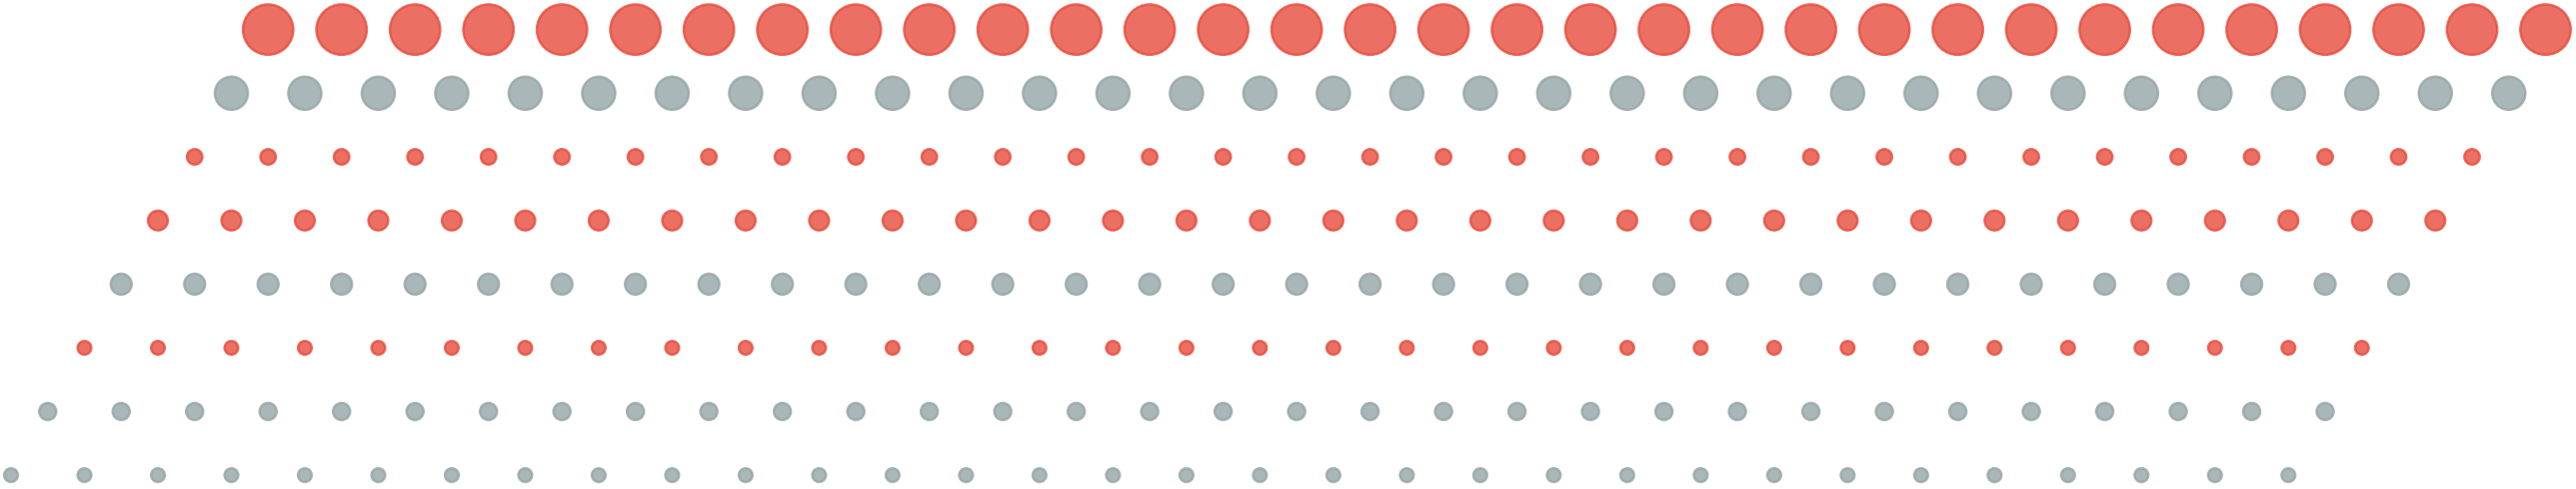
\includegraphics[scale=0.95]{Applications/MFnanoribbonTMD.png}
	\caption[Comparison between the MF solutions of the Hubbard model for a graphene nanoribbon (GNR) and a \acs{TMDNR}]{Comparison between the MF solutions of the Hubbard model at half filling for a graphene nanoribbon (GNR) at $U=1.2$ with $\beta t = 20$ (left) and a \acs{TMDNR} at $U=8$ (right), with $\beta | t_0 | = 20$.
	Both have $256$ sites.}
	\label{fig:nanoGraphVsTMD}
\end{figure}

\begin{figure}[H]
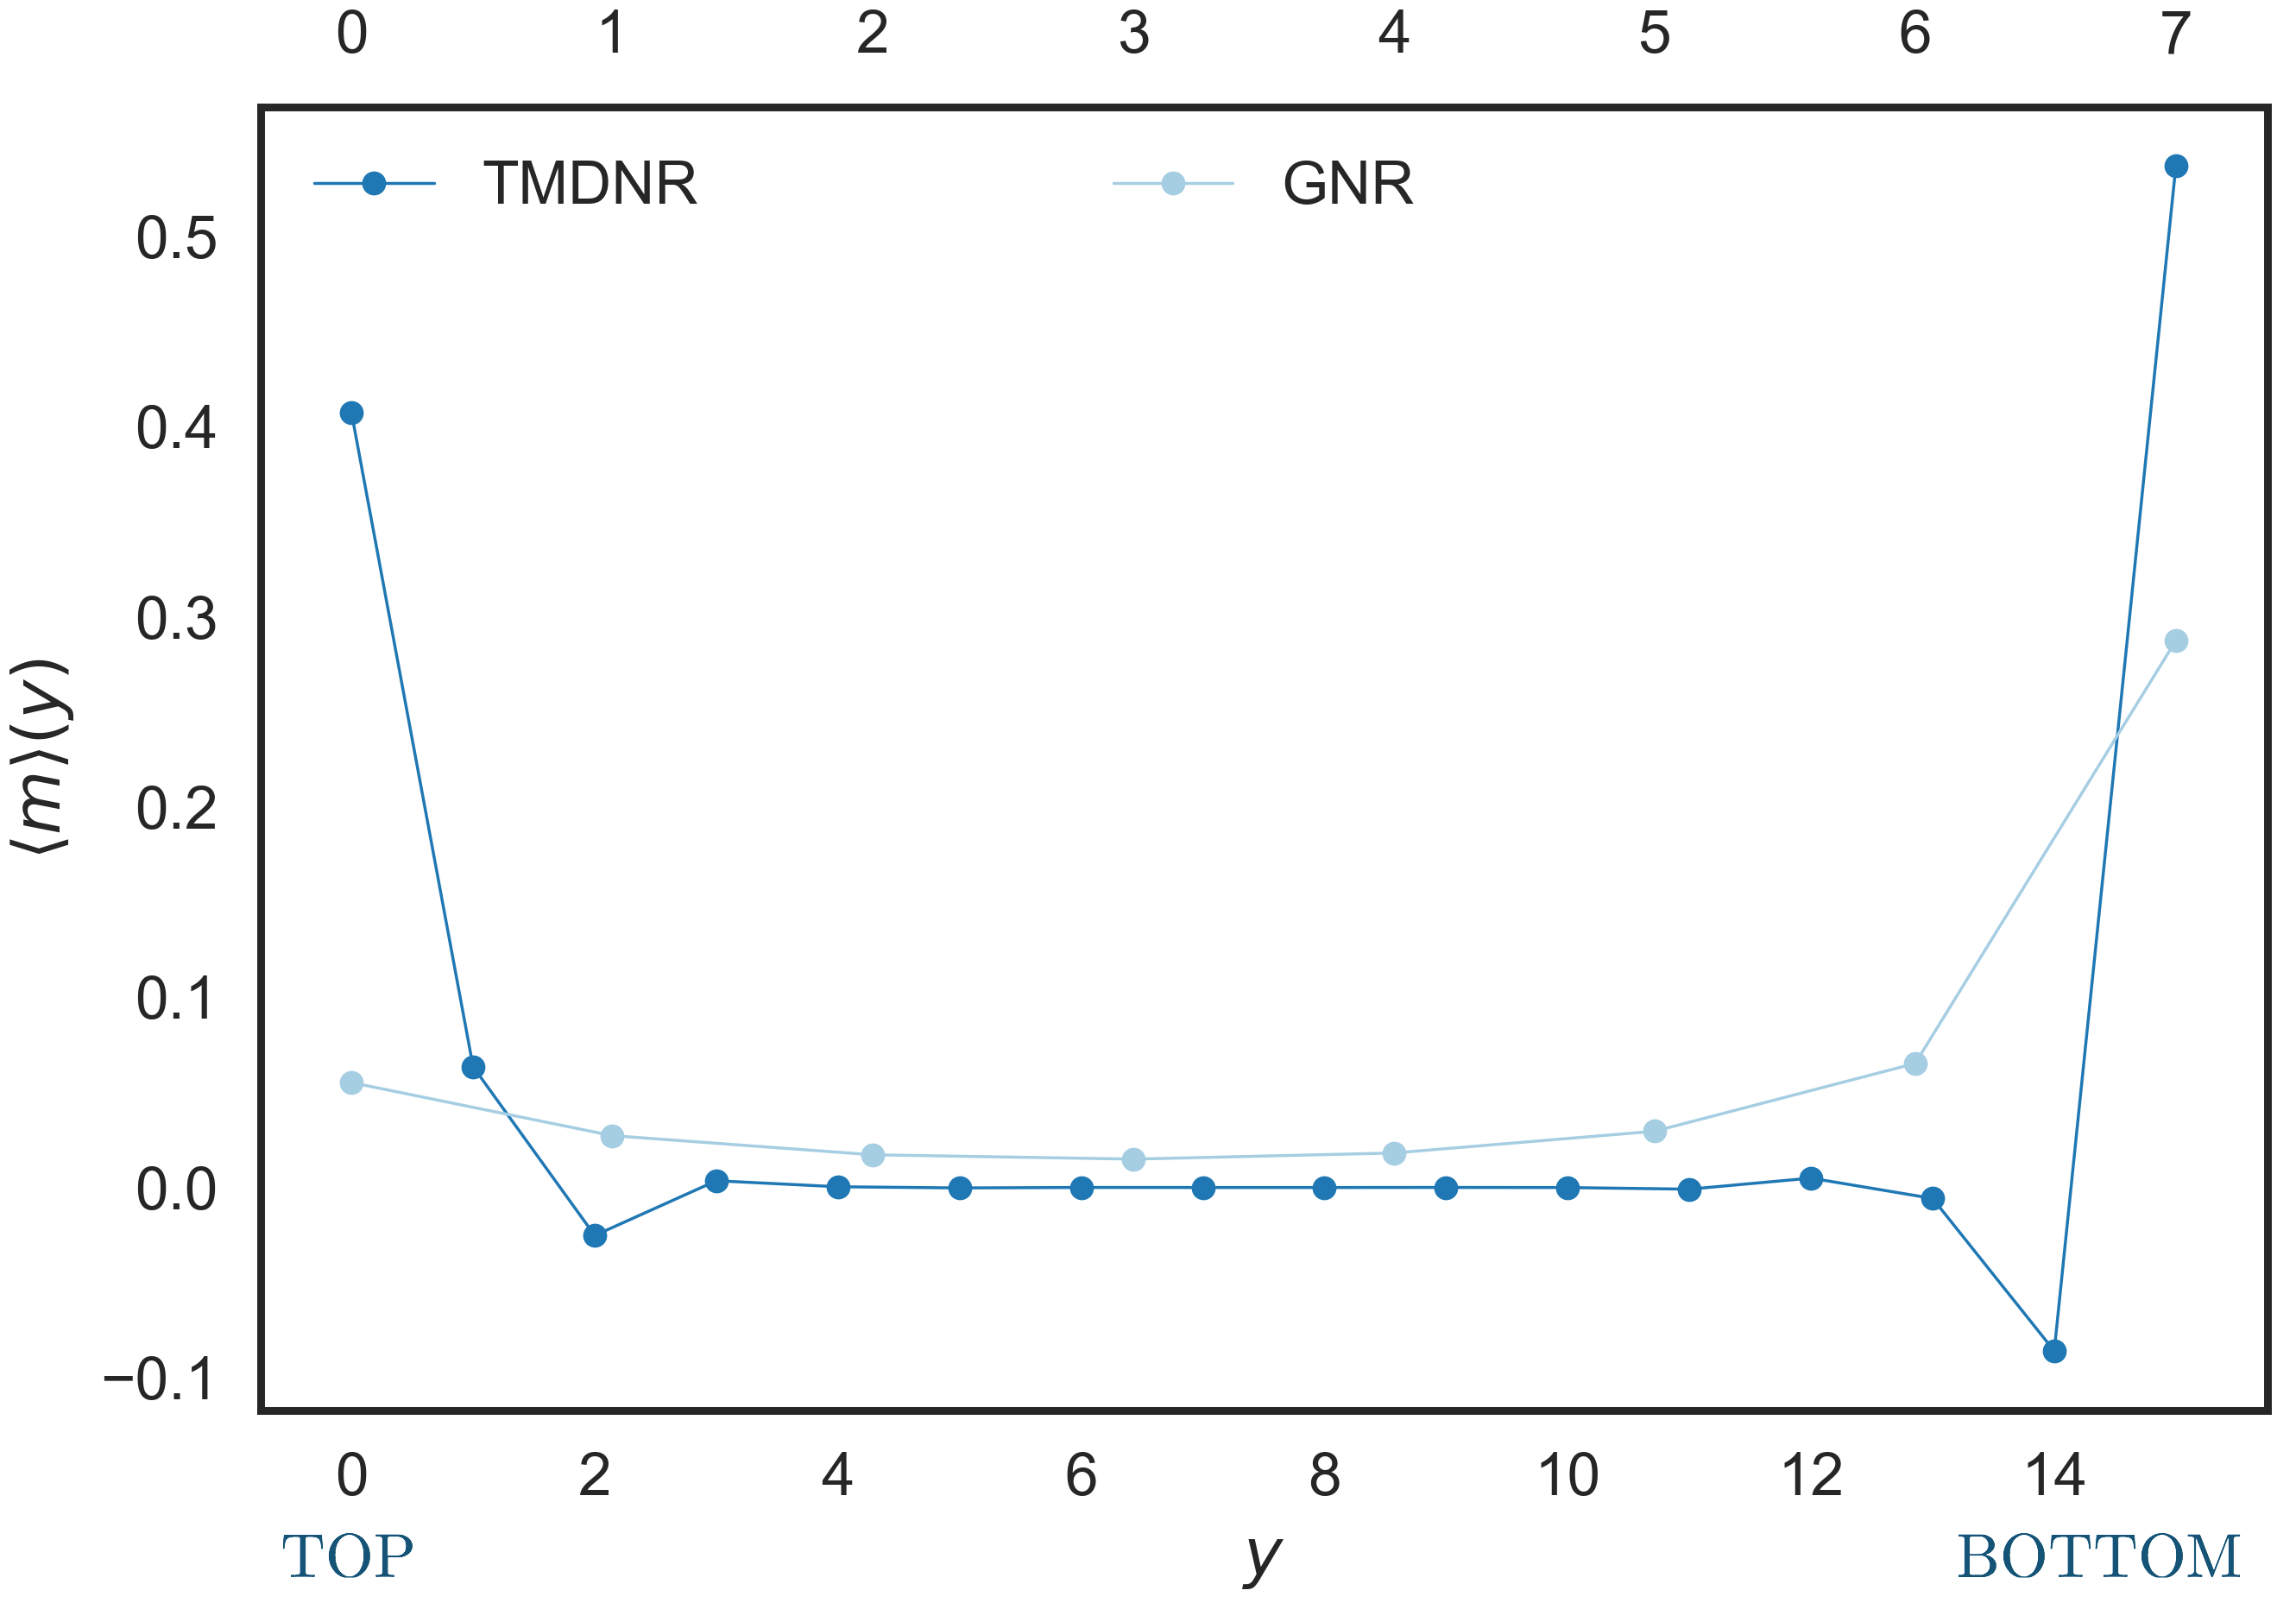
\includegraphics[scale=0.5]{Applications/magProf.png}
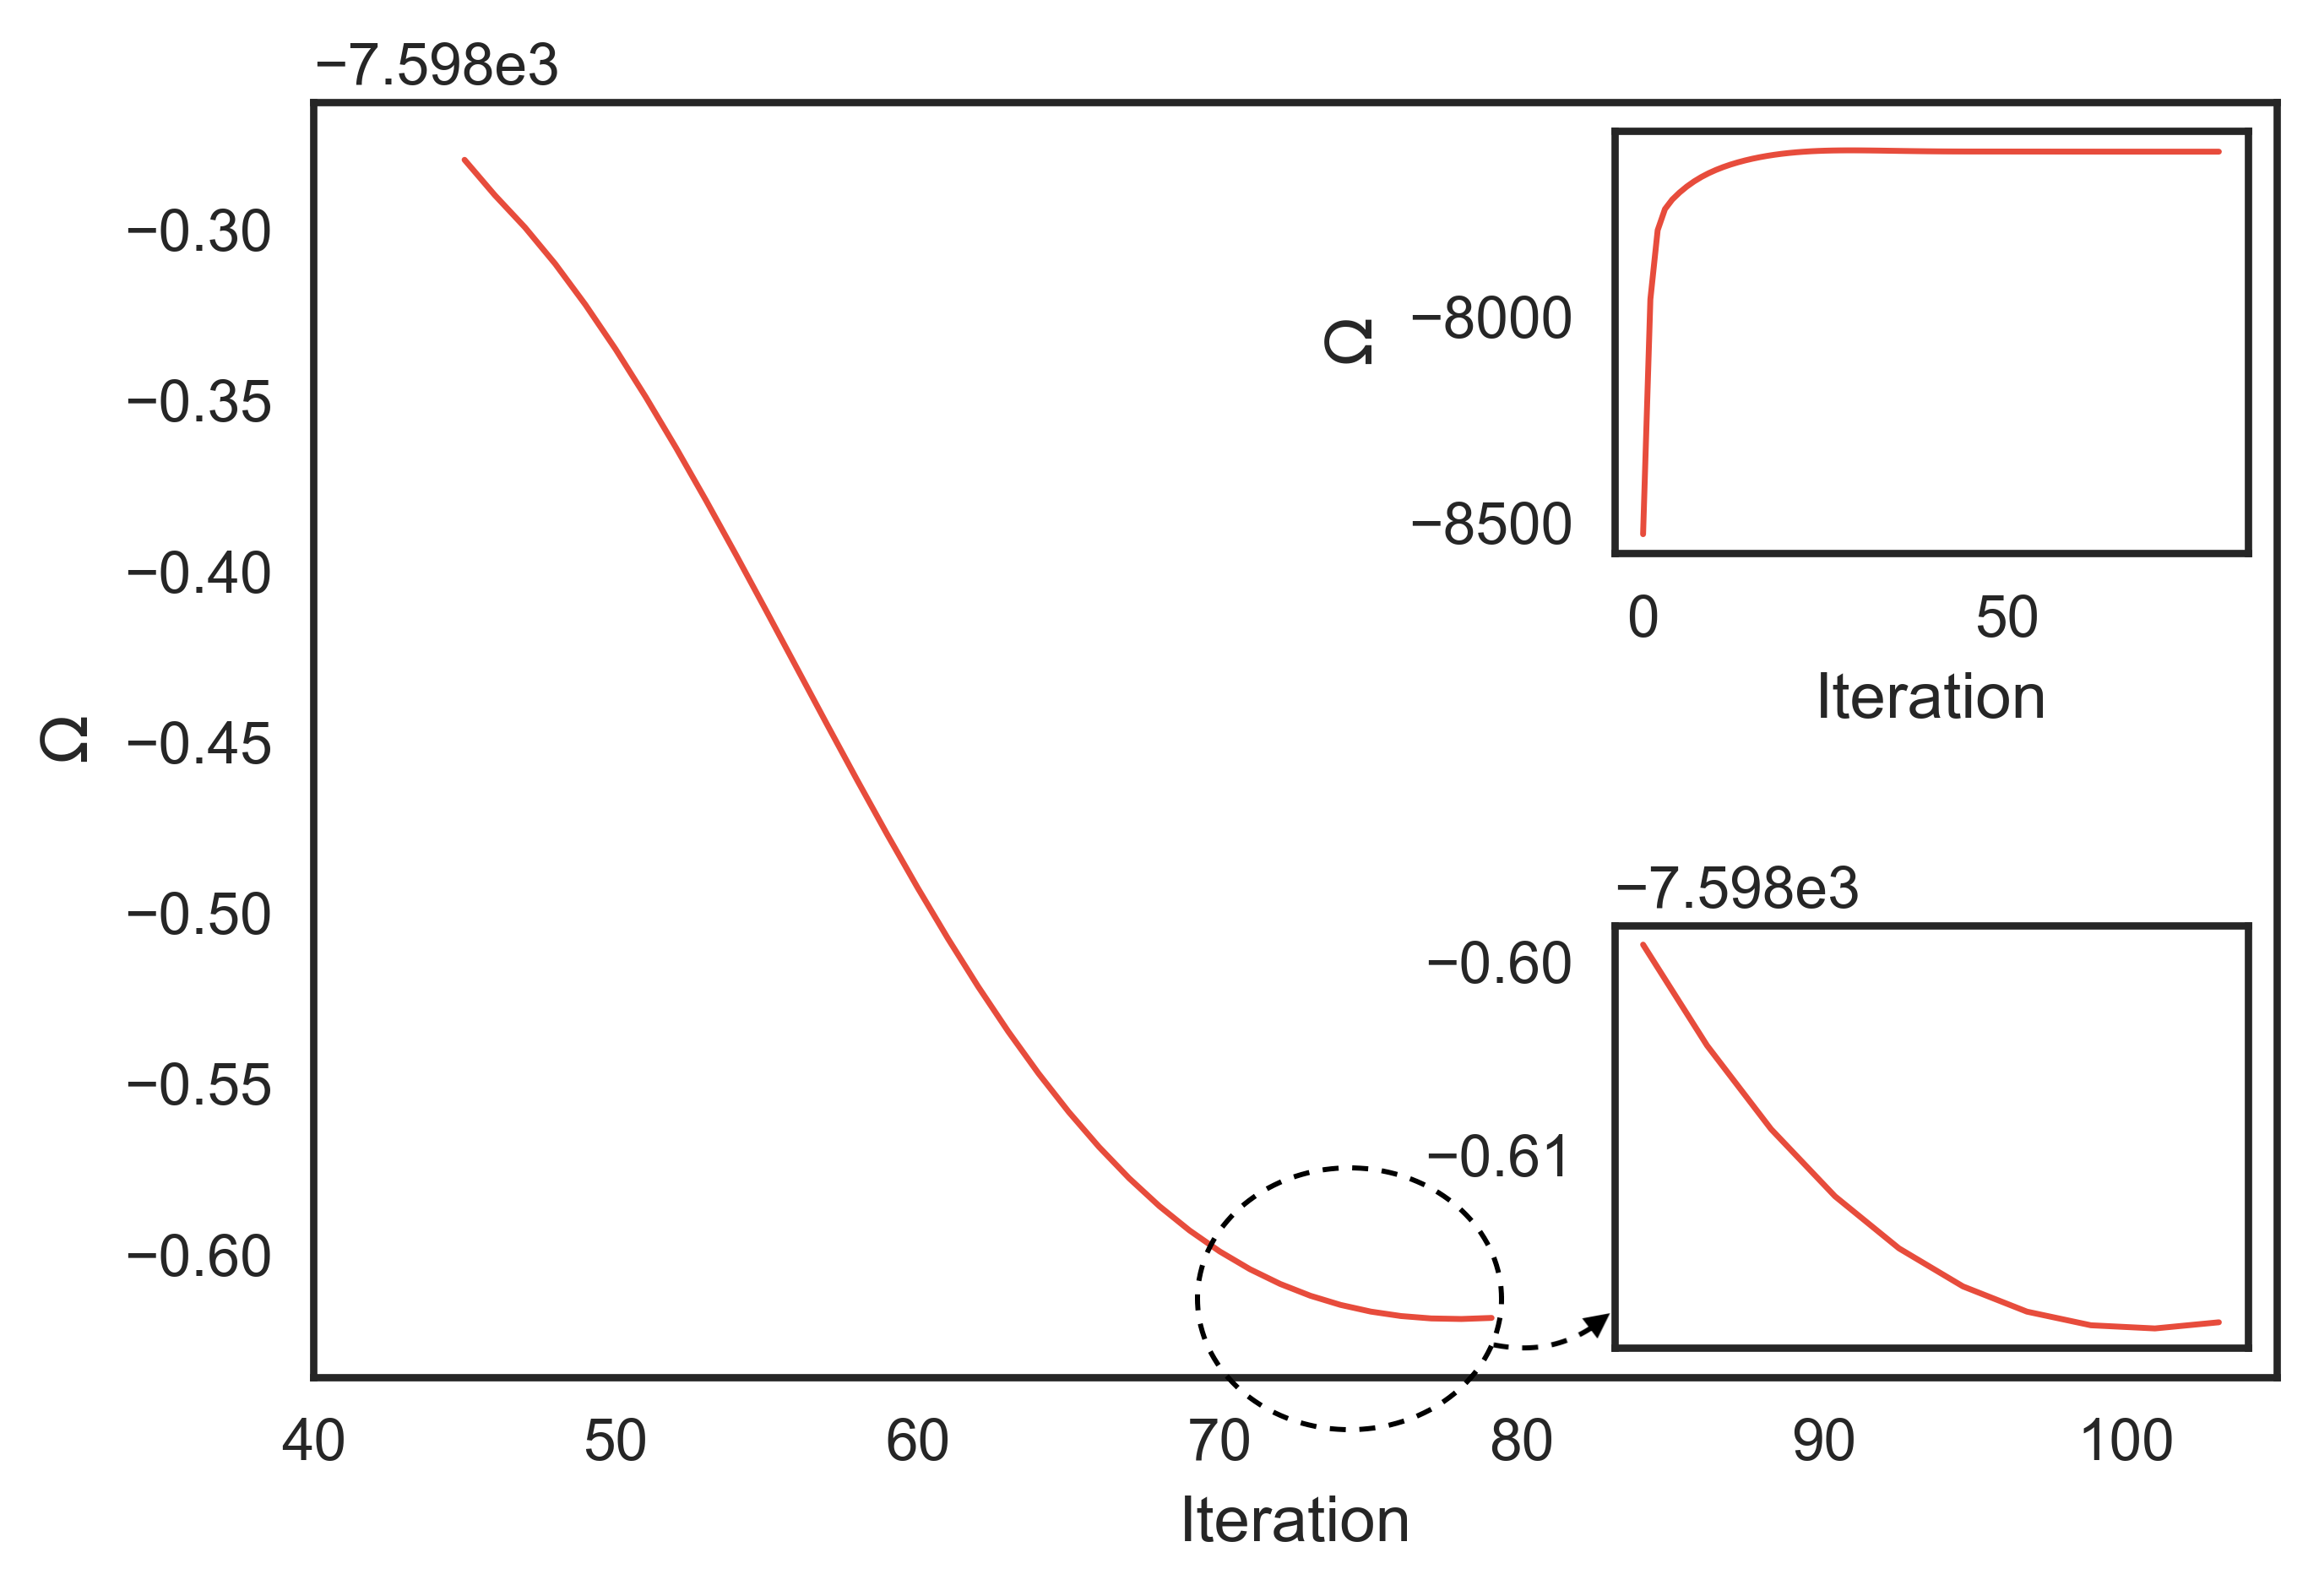
\includegraphics[scale=0.5]{Applications/grandPotMin.png}
	\caption[Spin density profile along the ribbon's transverse direction. Minimization of the grandpotential.]{Left: Spin density profile along the ribbon's transverse direction, with the inset showing that the obtained solution is constant along $x$. Right: Minimization of the grandpotential. 
	The upper inset shows that the grandpotential $\Omega$ initially increases due to the use of annealing to improve convergence. The main panel shows the behavior of $\Omega$ after the annealing phase has finished:
	$\Omega$ starts decreasing fast, then in the last iterations it stabilizes (as shown in the lower panel), and we consider that the self consistent solution has been achieved.}
	\label{fig:densSpinGrandPot}
\end{figure}

